\pror{} is the user interface of the Eclipse Requirements Modeling Framework.  This handbook strives to become a complete reference for \pror{}.  In addition, it will provide a tutorial, making it as easy as possible for new users to get started with requirements engineering.

\section{Conventions}

In this book, we use the following conventions:

% Formatted like remark
\begin{info}
Additional, useful information or tips are marked like this.
\end{info}

\begin{warning}
Warnings and marked like this.
\end{warning}

\begin{example}
Examples are marked like this.
\end{example}

When referring to \menu{menus} or \menu{user interface elements}, they are marked as shown here.

%\begin{definition}[Definition name]
%This is a definition
%\end{definition}

\section{Contributing}

Documentation is one of those things that gets easily neglected in open source projects.  It is also one of the easiest for outsiders to contribute to.  The documentation is managed as Latex, which may scare some people.  But no worries, those who don't want to learn Latex don't have to.

There are broadly two ways for contributing to the documentation:

\begin{description}
  \item[File a bug.]  Visit the \href{https://bugs.eclipse.org/bugs/enter_bug.cgi?assigned_to=&blocked=&bug_severity=normal&bug_status=NEW&comment=&contenttypeentry=&contenttypemethod=autodetect&data=&dependson=&description=&flag_type-1=X&flag_type-11=X&flag_type-12=X&flag_type-2=X&flag_type-4=X&flag_type-6=X&flag_type-7=X&flag_type-8=X&form_name=enter_bug&keywords=&&op_sys=All&product=MDT.RMF&qa_contact=&rep_platform=All&short_desc=&version=unspecified}{RMF Bug Tracker}.  You can just point out a problem or request for improvement.  You can also provide some text to be added to the documentation (unformatted).  If you do, however, then you need to sign a Committer License Agreement (CLA)
  \item[Submit improved \LaTeX via Gerrit.]  If you are technically inclined (meaning that you know what \LaTeX and git are, and how to use them), then you can contribute via the Gerrit code review system, as described \href{https://wiki.eclipse.org/Gerrit}{at eclipse.org}.
\end{description}

\subsection{Gerrit for Contributions}

TODO - when done, update the parent section as well.

\section{Licensed as EPL}

This work is licensed under the Eclipse Public License.

\section{Acknowledgements}

\begin{figure}
  \centering
  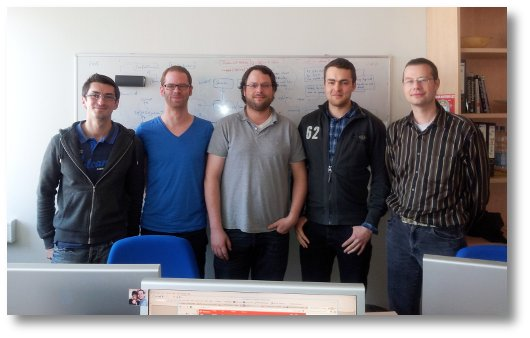
\includegraphics[width=\textwidth]{../rmf-images/2012_03_sprint_team.jpg}
  \caption{The RMF team during a Sprint in April 2012 in Düsseldorf, Germany}
  \label{fig:intro_core_team}
\end{figure}

Many parties were involved in creating RMF we would like to thank the core team that made it possible.

The roots of this project were created by Andreas Graf, Michael Jastram and Nirmal Sasidharan, who joined their various projects together.  Their efforts were financed by the research projects itea Verde and FP7 Deploy.  Together, they brought the project to the Eclipse Foundation, where it has been an active project ever since.  Figure~\ref{fig:intro_core_team} shows four of the five RMF Committers at a joint coding session (missing is Andreas Graf).


